\documentclass[addpoints,a4paper]{exam}

\usepackage{amsmath, amsfonts, amssymb, amsthm}
\usepackage{booktabs}
\usepackage{forest}
\usepackage{pythonhighlight}
\usepackage{tabularx}
\usepackage{tikz}
\usetikzlibrary{positioning}

\runningheader{CS 412 Algorithms}{Quiz 3A}{ID: \rule{.2\textwidth}{.5pt}}
\runningheadrule
\runningfootrule
\runningfooter{}{Page \thepage\ of \numpages}{}

% solution
\usepackage{draftwatermark}
\SetWatermarkText{Sample Solution}
\SetWatermarkLightness{.9}
\SetWatermarkScale{3}
\printanswers

\begin{document}
\begin{flushleft}
  { \large \textsf{\textbf{CS 412: Algorithms: Design and Analysis, L1, Quiz 3A, Spring 2023.}}}\vspace{.5em}
  
  \numquestions\ problems for \numpoints\ points on \numpages\ printed sides. Duration: 30 minutes. \today.
\end{flushleft}

Instructions:
\begin{enumerate}
  % \item Please observe the allowed time for this quiz as indicated on Canvas.
\item Enter your name and ID below and at the top of every side.
\item Solve the problems by hand in clear and legible handwriting in the provided space.
\item You may use the last side for rough work.
\item Provide precise and concise solutions.
\end{enumerate}

\noindent Student Name: \hrulefill \\[5pt]
\noindent Student ID: \hrulefill \\
\rule{\textwidth}{1pt}

\begin{questions}
  \question A \textit{contiguous subsequence} of a sequence $A$ is a sequence made up of consecutive elements of $A$. For instance, if $A = \langle5, 15, -30, 10, -5, 40, 10\rangle$ then $\langle15, -30, 10\rangle$ is a contiguous subsequence but $\langle5, 15, 40\rangle$ is not.

  We want to solve the following problem.

  \underline{Input}: A sequence, $A$, of numbers, $\langle a_1, a_2, \ldots, a_n\rangle$.\\
  \underline{Output}: A contiguous subsequence of $A$ that has maximum sum (the empty sequence has sum zero).
  
  For the preceding example, the answer would be $\langle10, -5, 40, 10\rangle$, with a sum of $55$.

  \begin{parts}
  \part[3] Characterize the structure of an optimal solution.\\
    \textit{Hint}: For each $i\in\{1,2,\ldots,n\}$, consider contiguous subsequences ending exactly at position $i$.
    \begin{solution}
      This is the first of the 4-step recipe to solve a problem using dynamic programming. The goal of the characterization is to demonstrate optimal substructure and overlapping subproblems.

      The problem is the same as the maximum subarray problem encountered previously in the divide-and-conquer module. Here, we employ a different approach to it, but use the same terminology for brevity.

      We note that the maximum subarray may contain negative numbers. As we scan it from left to right, the running sum may decrease but never becomes negative. This will not be achievable if, say, the given sequence only contains negative numbers. For this case, we use the property that the empty sequence, $\langle\rangle$, is always a subsequence. So the sum of the maximum subarray is always non-negative.

      There may be several subarrays with non-negative sum. We identify all of them as candidates, and denote as $C_i$ the candidate up to position $i$. The sum of $C_i$ is denoted as $S_i$. The maximum $S_i$ corresponds to the maximum subarray.

      There are two possibilities for $C_i$. One possibility is that it extends $C_{i-1}$, by appending $a_i$ to $C_{i-1}$. This happens when adding $a_i$ to the running sum so far, i.e. to $S_{i-1}$, yields a non-negative result.

      The other possibility occurs when adding $a_i$ to the running sum so far, i.e. to $S_{i-1}$, yields a negative result. In this case, $A_i$ is the empty sequence, $\langle\rangle$.

      For the base case, $C_0=\langle\rangle$.
      \[
        C_i = \begin{cases}
          \langle\rangle & i = 0\\
          C_{i-1}.append(a_i) & S_{i-1}+a_i \geq 0\\
          \langle\rangle & \text{otherwise}\\
        \end{cases}.
      \]
      $C_i$ depends on $C_{i-1}$ and on $S_{i-1}$ which also depends on $C_{i-1}$. This establishes optimal substructure. 
      The maximum subarray is the candidate with the maximum $S_i$. It requires each $S_i$ to be computed. The value of any $S_k$ is potentially required for computing every $S_i$ for $i> k$. This establishes overlapping subproblems.
    \end{solution}

    \part[2] Recursively define the value of an optimal solution.
      \begin{solution}
        We treat the sum of a maximum subarray as the value of an optimal solution. This is achieved through computing the sums of the candidates, $S_i$. A recursive expression for $S_i$ follows directly from the previous part.
      \[
        S_i = \begin{cases}
          0 & i = 0\\
          S_{i-1}+a_i & S_{i-1}+a_i \geq 0\\
          0 & \text{otherwise}\\
        \end{cases}.
      \]
      The value of the optimal solution is then the maximum $S_i$, i.e. $\max\{S_i \mid 1\leq i\leq n\}$.
      \end{solution}
    \part[3] Show how the value of an optimal solution can be computed in a bottom-up manner.
      \begin{solution}
        \ \newline
        \begin{tabularx}{\linewidth}{X|c}
          We see in the recurrence above that $S_i$ depends on $S_{i-1}$. The resulting problem subgraph is shown on the right.

          $S_n$ can then be computed as follows. $S_0$ is initialized, which then enables to compute, $S_1$, which then enables $S_2$, and so on. This can be achieved by running a loop from $i=1$ to $i=n$.

          The value of the optimal solution can be computed by maintaining a variable for the maximum $S_i$ seen so far and updating it with the computed $S_i$ in each iteration.
          &
          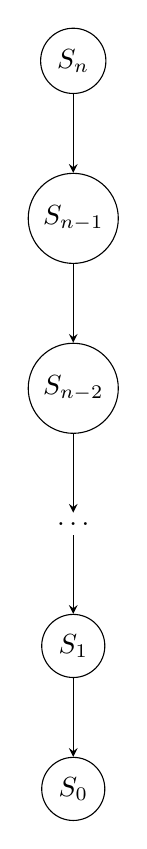
\begin{tikzpicture}[baseline=(n-1)]
            \node[draw,circle] (n) at (0,0) {$S_n$};
            \node[draw,circle] (n-1)[below=of n] {$S_{n-1}$};
            \node[draw,circle] (n-2)[below=of n-1)] {$S_{n-2}$};
            \node (e)[below=of n-2)] {$\ldots$};
            \node[draw,circle] (1)[below=of e)] {$S_1$};
            \node[draw,circle] (0)[below=of 1)] {$S_0$};

            \draw[-stealth] (n) -- (n-1);
            \draw[-stealth] (n-1) -- (n-2);
            \draw[-stealth] (n-2) -- (e);
            \draw[-stealth] (e) -- (1);
            \draw[-stealth] (1) -- (0);
          \end{tikzpicture}
        \end{tabularx}
      \end{solution}
  \part[2] Argue about the time and space complexities of your approach.
    \begin{solution}
      The approach above involves iterating over the sequence $A$ once and doing a constant amount of work in each iteration. It thus has a time complexity of $\Theta(n)$.

      $A$ needs to be stored and accessed, which requires $\Theta(n)$ space. If that is overlooked, we can reason about  the space overhead just for the computation as follows.

      The computation requires access to all $S_i$ values for $1\leq i\leq n$. This requires $\Theta(n)$ space. In fact, we can do without storing all $S_i$ values, by noting that only the previous $S_i$ is required in a given iteration. This can be stored in a single variable which is updated in each iteration. With this approach, the computation requires just $\Theta(1)$ space.
    \end{solution}
  \end{parts}
\end{questions}

\newpage
\centerline{\large Rough Work}

\end{document}

%%% Local Variables:
%%% mode: latex
%%% TeX-master: t
%%% End:
